% Created 2023-03-03 ven. 22:23
% Intended LaTeX compiler: pdflatex
\documentclass[11pt]{article}
\usepackage[utf8]{inputenc}
\usepackage[T1]{fontenc}
\usepackage{graphicx}
\usepackage{grffile}
\usepackage{longtable}
\usepackage{wrapfig}
\usepackage{rotating}
\usepackage[normalem]{ulem}
\usepackage{amsmath}
\usepackage{textcomp}
\usepackage{amssymb}
\usepackage{capt-of}
\usepackage{hyperref}
\usepackage{lmodern} % Ensures we have the right font
\usepackage{graphicx}
\usepackage{amsmath, amsthm, amssymb}
\usepackage[table, xcdraw]{xcolor}
\usepackage{fancyhdr}
\usepackage[lined,boxed,commentsnumbered,ruled,vlined,linesnumbered]{algorithm2e}
\SetKwComment{Comment}{$\triangleright$\ }{}
\usepackage[left=2cm,right=2cm,top=3cm,bottom=3cm]{geometry}
\pagestyle{fancy}
\fancyhf{}
\lhead{Modify in current org file : \lhead{foo}}
\rfoot{Page \thepage}
\usepackage{titling}
\setlength{\droptitle}{-8ex}
\pretitle{\begin{flushleft}\Large\bfseries}
\posttitle{\par\end{flushleft}}
\preauthor{\begin{flushleft}\large}
\postauthor{\end{flushleft}}
\predate{\begin{flushleft}}
\postdate{\end{flushleft}}
\usepackage[normalem]{ulem}
\usepackage{sectsty}
\sectionfont{\underline}
\makeatletter
\def\@seccntformat#1{%
\expandafter\ifx\csname c@#1\endcsname\c@section\else
\csname the#1\endcsname\quad
\fi}
\makeatother
\definecolor{bblue}{HTML}{275382}
\usepackage[colorlinks]{hyperref}
\hypersetup{colorlinks, linkcolor=bblue, urlcolor=bblue}
\usepackage[font={color=gray},figurename=Fig.,labelfont={it}]{caption}
\usepackage{enumitem}
\setlist{noitemsep}
\renewcommand{\contentsname}{Sommaire}
\usepackage{listings}
\usepackage{tikz}
\usepackage{lstautogobble}  % Fix relative indenting
\usepackage{color}          % Code coloring
\usepackage{zi4}            % Nice font
\definecolor{bluekeywords}{rgb}{0.13, 0.13, 1}
\definecolor{greencomments}{rgb}{0, 0.5, 0}
\definecolor{redstrings}{rgb}{0.9, 0, 0}
\definecolor{graynumbers}{rgb}{0.5, 0.5, 0.5}
\definecolor{grayW}{rgb}{0.96,0.96,0.97}
\usepackage{listings}
\lstset{
backgroundcolor=\color{grayW},
autogobble,
columns=fullflexible,
showspaces=false,
showtabs=false,
breaklines=true,
showstringspaces=false,
breakatwhitespace=true,
escapeinside={(*@}{@*)},
commentstyle=\color{greencomments},
keywordstyle=\color{bluekeywords},
stringstyle=\color{redstrings},
numberstyle=\color{graynumbers},
basicstyle=\ttfamily\footnotesize,
frame=tlbr,
framesep=12pt,
xleftmargin=12pt,
tabsize=4,
captionpos=b,
framexleftmargin=15pt,
framerule=0pt
}
\lhead{DUREL Enzo, VILLEPREUX Thibault}
\rhead{SDD TP1: Polynomes}
\usepackage{listings}
\author{DUREL Enzo, VILLEPREUX Thibault}
\date{\today}
\title{SDD TP1: Polynomes}
\hypersetup{
 pdfauthor={DUREL Enzo, VILLEPREUX Thibault},
 pdftitle={SDD TP1: Polynomes},
 pdfkeywords={},
 pdfsubject={},
 pdfcreator={Emacs 27.1 (Org mode 9.3)}, 
 pdflang={English}}
\begin{document}

\maketitle
\tableofcontents

\thispagestyle{fancy}

\newpage

\section{Présentation}
\label{sec:org54afc19}
Notre objectif principal est de pouvoir construire des fonctions de base pour manipuler
des polynômes. Nous essayons donc de nous rapprocher le plus possible de la
programmation modulaire avec les contraintes du langage C, pour pouvoir importer
par la suite notre objet polynôme dans d'autres projets.

Nous pouvons retrouver comme fonctions de base :
\begin{itemize}
\item la dérivation d'un polynôme,
\item l'addition de deux polynômes
\item et la multiplication de deux polynômes.
\end{itemize}

Un polynôme est stocké sous forme d'une liste simplement chaînée (aussi appelé linkedlist) de monôme. Il
est donc nécessaire, de créer aussi des fichiers contenant des fonctions pour
manipuler des listes simplement chaînées, et des fichiers pour manipuler des
monômes, afin de respecter l'approche de la programmation modulaire.

De plus, les maillons de la liste simplement chaînée sont rangés par ordre de
degré croissant et il ne peut pas y avoir deux monômes différents avec un même
degré, ou un monôme avec un coefficient nul.

Il nous a été imposé de représenter des polynômes avec une
linkedlist plutôt qu'avec un tableau pour les avantages suivants :
\begin{itemize}
\item gérer la flexibilité de la taille plus facilement, exemple : avec la
\end{itemize}
multiplication, le degré du polynôme peut être très vite élevé
\begin{itemize}
\item une meilleure complexité dans beaucoup de cas, exemple : pour insérer lors de l'addition
\end{itemize}
pas d'appel de decaleGauche ou de  decaleDroite sur un tableau, insertion en
O(1) pour une linkedlist car on connaît le précédent
\begin{itemize}
\item gain en complexité spaciale : on ne représente pas les monômes de coefficient nul
\item facilité de manipulation : insertion et suppression plus facile par exemple
\end{itemize}

Dans la suite du rapport, nous expliquerons les structures de données, et détaillerons
les principes des fonctions. 

\section{Structures de Données}
\label{sec:org7e918b9}

\subsection{Description}
\label{sec:org4624cf5}
\subsubsection{Monôme}
\label{sec:org4f7efb3}
Un monôme est stocké sous forme d'une structure en C, son type est \textbf{monom\textsubscript{t}}.

Cette structure possède deux champs :
\begin{itemize}
\item un champ coef, de type double, qui représente comme son nom l'indique le
\end{itemize}
coefficient du monôme.
\begin{itemize}
\item un champ degree, de type unsigned int, qui représente comme son nom
\end{itemize}
l'indique le degré du monôme. Nous avons fait le choix de choisir une variable
non signée afin de provoquer une erreur dans le programme si le degré devient
négatif, car le polynôme ne doit pas avoir de degré négatif. Ainsi, nous
pourrons en théorie stocker des degrés de taille un bit plus grand.

\subsubsection{Liste Simplement Chainnée}
\label{sec:org7acf763}

Une liste simplement chaînée ou linkedlist est stockée sous forme de structure, son type est
\textbf{cell\textsubscript{t}}.

Cette structure possède deux champs :
\begin{itemize}
\item un champ val, de typage monom\textsubscript{t}, qui représente les informations stockées sous
\end{itemize}
la forme d'un monôme. 
\begin{itemize}
\item un champ next, de typage cell\textsubscript{t} *, qui représente un pointeur vers le maillon
\end{itemize}
suivant du maillon actuel.

Pour résumer, chaque maillon de la liste possède trois informations :
\begin{itemize}
\item le degré du monôme du maillon
\item le coefficient du monôme du maillon
\item et un pointeur vers le prochain maillon, qui peut être NULL si le maillon
\end{itemize}
courant est le dernier de la liste.


\subsubsection{Polynôme}
\label{sec:orgee27d91}

Un polynôme est une liste simplement chaînée. Il n'y a pas de structure
polynôme spécialement défini.

Le fichier source \textbf{polynome.c} possède seulement des fonctions pour manipuler cet
objet. Et c'est grâce à ces dernières, que l'on peut garantir de l'unicité d'un
maillon pour le degré monôme, ou la bonne insertion d'un monôme dans le
polynôme, en respectant l'ordre de degré croissant par exemple.

\subsection{Schéma}
\label{sec:org17e4438}
s

Voici le schéma d'un polynôme non vide:
\begin{verbatim}
+------+       +-------+-------+-------+       +-------+-------+-------+
|      |       |       |       |       |       |       |       |       |
|      +------>|       |       |       +------>|       |       |       +------> ...
|      |       |       |       |       |       |       |       |       |
+------+       +-------+-------+-------+       +-------+-------+-------+
   a0	          deg    coeff   next             deg    coeff   next
	       +-------+-------+		    
		       |			    
		     monom
\end{verbatim}

Voici le schéma d'un polynôme vide:
\begin{verbatim}
+------+
|      |
| NULL |
|      |
+------+
   a0	  
\end{verbatim}
\begin{center}
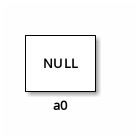
\includegraphics[width=.9\linewidth]{img/structure_cell_empty.png}
\end{center}

On retrouve les cases mémoires expliquées précédemment comme le degré d'un monôme, le
coefficient d'un monôme, et le pointeur next de la liste chainée.
La variable a0 quand à elle est un pointeur vers le premier maillon du
polynome/linkedlist. De plus, le contenu de la case next du dernier maillon vaut NULL.

\subsection{Fichiers de données}
\label{sec:orgf318a46}

La mise en place de tests unitaires a permis de vérifier la validité des
fonctions, en détectant les erreurs dans le comportement des fonctions isolées,
ce qui a contribué à améliorer la qualité et la fiabilité du code.

Afin de garantir une couverture la plus complète possible de toutes les
situations et des différents cas d'utilisation, nous avons utilisé divers
fichiers de test. Ces fichiers sont présents dans /src/data.

Les fichiers que l'on a créés sont :
\begin{itemize}
\item poly1.txt à poly9.txt : pour les tests dans polynomial\textsubscript{main.c}.
\item listeChainneeTest.txt : pour les tests dans linkedlist\textsubscript{main.c}, il y a un seul
\end{itemize}
fichier test car on fait beaucoup d'insertion à la main, pour tester la fonction
LL\textsubscript{add}\textsubscript{cell}.


\section{Architecture}
\label{sec:org4c30304}

Dans le dossier \textbf{zz1\textsubscript{sdd}\textsubscript{tp1}} se trouve plusieurs fichiers et répertoires.
Il y a :
\begin{itemize}
\item le répertoire \textbf{rapport} qui contient le rapport en pdf.
\item le répertoire \textbf{src} qui contient l'ensemble des fichiers de code et qui
\end{itemize}
contient à son tour le répertoire \textbf{data} avec tous les fichiers de test 
\begin{itemize}
\item le fichier readme
\end{itemize}

Comme expliqué précédemment, afin de manipuler les polynômes, nous avons créé un
objet monôme et un objet linkedlist.

Les fonctions pour manipuler des monômes se trouve dans \textbf{valCell.c} et leurs
prototypes dans \textbf{valCell.h}.

Les fonctions pour manipuler des linkedlist se trouve dans \textbf{linkedList.c} et leurs
prototypes dans \textbf{linkedList.h}.

Il y a aussi le fichier \textbf{linkedlist\textsubscript{main.c}} qui contient les tests unitaires
pour certifiée la validité des méthodes.


\section{Fonctions}
\label{sec:orgdaf0c5c}
\subsection{linkedList}
\label{sec:org3a18322}
\subsubsection{LL\textsubscript{init}\textsubscript{list}}
\label{sec:org1405ec5}
\begin{enumerate}
\item Description
\label{sec:org77d09cc}

\begin{verbatim}
La fonction initialise la liste à NULL.
\end{verbatim}

\item Algorithme
\label{sec:org619528c}

\begin{verbatim}
\begin{algorithm}
  \caption{Procédure d'initialisation d'une liste}\label{alg:two}
  \KwData{ES: adrHeadPt$}
  $adrHeadPt \gets NIL$\;
\end{algorithm}
\end{verbatim}

\item Signature
\label{sec:org81064df}

\begin{verbatim}
void LL_init_list(cell_t **adrHeadPt);
\end{verbatim}

\item Code source
\label{sec:org2a071c5}

\begin{verbatim}
 1  /**
 2   * @fn void LL_init_list(cell_t **adrHeadPt)
 3   * @brief Initialize a void list
 4   * @param [in, out] adrHeadPt address of head pointer of the list 
 5   */
 6  void LL_init_list(cell_t **adrHeadPt)
 7  {
 8      // initialise la liste a NULL
 9      *adrHeadPt = NULL;
10  }
\end{verbatim}

\item Lexique
\label{sec:org385b35a}
\begin{enumerate}
\item Paramètres
\label{sec:org4817ee6}
\begin{itemize}
\item \texttt{cell\_t ** adrHeadPt}: adresse du pointeur de tête de liste
\end{itemize}
\item Variables
\label{sec:orge0327e9}
\begin{itemize}
\item Aucune variable dans cette fonction.
\end{itemize}
\end{enumerate}
\end{enumerate}


\subsubsection{LL\textsubscript{create}\textsubscript{cell}}
\label{sec:orgfa2b847}
\begin{enumerate}
\item Description
\label{sec:orgba9c0ab}

\begin{verbatim}
La fonction créée et initialise une nouvelle cellule. Elle renvoie NULL si
l'allocation a échoué, sinon l'adresse de la cellule allouée.
\end{verbatim}

\item Algorithme
\label{sec:org0d4401a}

\begin{verbatim}
\begin{algorithm}
  \caption{Fonction de création de cellule}\label{alg:two}
  \KwData{E: $pmonome \neq NIL$}
  $new \gets NIL$\;
  $new \gets alloc(taille(cellule))$\;
  \If{$new \neq NIL$}{
    $m(coef(new)) \gets coef(pmonome)$\;
    $m(degree(new)) \gets degree(pmonome)$\;
    $m(next(new)) \gets NIL$\;
  }
  \Return{$new$\;}
\end{algorithm}
\end{verbatim}

\item Signature
\label{sec:orgb8cdc11}

\begin{verbatim}
cell_t * LL_create_cell(monom_t * pmonome);
\end{verbatim}

\item Code source
\label{sec:orge8ce3de}

\begin{verbatim}
 1  /** 
 2   * @brief create a new cell for linked list from its data 
 3   * @param [in] pdata address of the data
 4   * @return address of the new cell
 5   */
 6  cell_t * LL_create_cell(monom_t * pmonome)
 7  {
 8      cell_t * new = NULL;
 9      // alloue dynamiquement le monome
10      new = (cell_t *) malloc(sizeof(cell_t));
11      // si l'alloc a fonctionnee 
12      if (NULL != new)
13      {
14  	new->val.coef    = pmonome->coef;   //init le coef
15  	new->val.degree  = pmonome->degree; //init le degre
16  	new->next        = NULL;            //init le suivant
17      }
18  
19      return new; // retrun NULLsi erreur malloc
20  }
21  
\end{verbatim}

\item Lexique
\label{sec:org6f75b4c}
\begin{enumerate}
\item Paramètres
\label{sec:orge1193e6}
\begin{itemize}
\item \texttt{monom\_t * pmonome}: adresse du monome à ajouter à la liste.
\end{itemize}
\item Variables
\label{sec:org069a3c7}
\begin{itemize}
\item \texttt{cell\_t * new}: pointeur vers la nouvelle cellule créée.
\end{itemize}
\end{enumerate}
\item Hypothèse
\label{sec:orge18f7ea}
Le monôme n'est pas NULL et contient des valeurs cohérentes. Par exemple, si on l'utilise pour
représenter des polynômes, le coefficient n'est pas nul et le degré est positif.
\end{enumerate}


\subsubsection{LL\textsubscript{add}\textsubscript{cell}}
\label{sec:org209b626}
\begin{enumerate}
\item Description
\label{sec:orgbb1c06b}

\begin{verbatim}
La fonction ajoute une cellule à une liste à partir d'un précédent.
\end{verbatim}

\item Algorithme
\label{sec:orge0e2493}

\begin{verbatim}
\begin{algorithm}
  \caption{Procédure d'ajout de cellule}\label{alg:two}
  \KwData{ES: $a \neq NIL$, $prec \neq NIL$}
  $next(a) \gets cm(prec)$\;
  $m(cm(prec)) \gets a$\;
\end{algorithm}
\end{verbatim}

\item Signature
\label{sec:org48525ad}

\begin{verbatim}
void LL_add_cell(cell_t ** prec, cell_t * a);
\end{verbatim}

\item Code source
\label{sec:org0ff1792}

\begin{verbatim}
 1  /**
 2   * @brief Insert a cell into a linked list at the given position
 3   * @param [in, out]  prec address of previous pointer of the cell
 4   * @param [in]  a address of the cell to be added to the linked list
 5   */
 6  void LL_add_cell(cell_t ** prec, cell_t * a)
 7  {
 8      a->next = *prec; // modifie le suivant du maillon qu'on insert
 9      *prec   = a;     // realise le chainge avec prec
10  }
\end{verbatim}

\item Lexique
\label{sec:orgb036e97}
\begin{enumerate}
\item Paramètres
\label{sec:org774751e}
\begin{itemize}
\item \texttt{cell\_t * a}: adresse de la cellule à ajouter.
\item \texttt{cell\_t ** prec}: adresse de la cellule qui précède à après ajout.
\end{itemize}
\item Variables
\label{sec:orgdcb2bcc}
\begin{itemize}
\item Aucune variable dans cette fonction.
\end{itemize}
\end{enumerate}

\item Hypothèse
\label{sec:org2085350}
La cellule que l'on ajoute a été allouée précédemment, elle ne peut pas être NULL.
\item Liste des cas
\label{sec:orgb117f66}
LL\textsubscript{add}\textsubscript{cell} quand :
\begin{itemize}
\item la liste est vide
\item il faut insérer au milieu de liste
\item il faut insérer en tête de liste
\item il faut insérer en fin de liste
\end{itemize}
\end{enumerate}

\subsubsection{LL\textsubscript{create}\textsubscript{list}\textsubscript{fromFileName}}
\label{sec:orgf80d280}
\begin{enumerate}
\item Description
\label{sec:org3efa346}

\begin{verbatim}
La fonction créée une liste à partir d'un nom d'un fichier. Si le fichier
n'a pas réussi à être ouvert, la liste sera vide. Si une erreur d'allocation a
lieu lors de la création des maillons pendant la lecture du fichier, la
liste sera libérée proprement et la fonction renverra la liste vide.
\end{verbatim}

\item Algorithme
\label{sec:orgedde225}

\begin{verbatim}
\begin{algorithm}
  \caption{Fonction de création de liste à partir d'un nom de fichier}\label{alg:two}
  \KwData{E: $filename$, ES: $a0$}
  $ouvrir(filename)$\;
  \While{non fin(filename)}{
      $m(mread) \gets lireMonome(filename)$\Comment*{Lit le monome dans le fichier}
      $m(curr) \gets creerCellule(mread)$\;
      $m(prec) \gets chercherPrecedent(curr, pfcmp)$\;
      $ajouterCellule(prec, curr)$\;
  }
  \Return{$a0$}\;
\end{algorithm}
\end{verbatim}

\item Signature
\label{sec:org70557b8}

\begin{verbatim}
cell_t ** LL_create_list_fromFileName(cell_t ** a0,
				      char * fname,
				      int (*pfcmp) (monom_t *, monom_t *));
\end{verbatim}

\item Code source
\label{sec:orgfd7e1df}

\begin{verbatim}
 1  /**
 2   * @brief Create a linked list from a file
 3   * @param [in, out] a0 address of head pointer of a linked list
 4   * @param [in] fname name of a file containing the data for a linked list
 5   * @param pfcmp fonction pointer for comparison of two cell's value
 6   * @return head pointer of the linked list
 7   */
 8  cell_t ** LL_create_list_fromFileName(cell_t ** a0,
 9  				      char * fname,
10  				      int (*pfcmp) (monom_t *, monom_t *))
11  {
12      FILE   *  fp    = fopen(fname, "r"); // si fname = NULL alors fp := NULL 
13      cell_t ** prec  = NULL;
14      cell_t *  curr  = NULL;
15      int  error      = 0 ;                // = 1 si erreur malloc
16      monom_t   mread;
17  
18      LL_init_list(a0);
19  
20      if (NULL != fp) { // ouverture fichier OK
21  	//lire une ligne
22  	while ( 2 ==  fscanf(fp, "%lg %d\n", &mread.coef, &mread.degree )
23  		&& !error)
24  	{
25  	    //créer cellule
26  	    curr = LL_create_cell(&mread);
27  
28  	    if (NULL != curr) // si malloc reussi
29  	    {
30  		//insérer cellule
31  		prec = LL_search_prev(a0, &mread, pfcmp);
32  		LL_add_cell(prec, curr);
33  	    }
34  	    else //message erreur malloc + free liste
35  	    {
36  		error = 1;
37  		fprintf(stderr,
38  			"%s : Erreur problème lors de l'allocation : %s\n",
39  			__FUNCTION__,
40  			fname);
41  		// libere toute la liste en cas d'erreur
42  		LL_free_list(a0);
43  	    }	
44  	}
45  	fclose(fp);
46      }
47      else { // message erreur ouverture
48  	fprintf(stderr,
49  		"%s : 'Erreur lors de l'ouverture du fichier: %s'\n",
50  		__FUNCTION__,
51  		fname);
52      }
53      return a0; // retourne la liste
54  }
\end{verbatim}

\item Lexique
\label{sec:org89cf582}
\begin{enumerate}
\item Paramètres
\label{sec:org8aa7559}
\begin{itemize}
\item \texttt{char * filename}: nom du fichier.
\item \texttt{cell\_t ** a0}: pointeur vers le début de la liste.
\item \texttt{int * pfcmp (monom\_t* , monom\_t* )}: pointeur de fonction qui compare les monomes en paramètres.
\end{itemize}
\item Variables
\label{sec:org54b4582}
\begin{itemize}
\item \texttt{cell\_t * curr}: adresse de la cellule lue.
\item \texttt{cell\_t ** prec}: adresse de la cellule qui précède lue d'après la fonction de comparaison.
\item \texttt{FILE * fp}: fichier de lecture.
\item \texttt{int * error}: erreur d'allocation de la mémoire pour curr.
\item \texttt{monom\_t mread}: monome qui est lu dans le fichier et qui sert à créer la cellule.
\end{itemize}
\end{enumerate}

\item Hypothèse
\label{sec:org8e4e526}
La fonction pfcmp existe et elle est utilisable/fonctionelle.

\item Liste des cas
\label{sec:orgdceb8cb}
LL\textsubscript{create}\textsubscript{liste}\textsubscript{fromFileName} foncitonne quand :
\begin{itemize}
\item le fichier n'existe pas
\item le fichier est vide
\item le fichier contient des lignes sous la forme suivante : "double entier \n"
\end{itemize}
\end{enumerate}

\subsubsection{LL\textsubscript{save}\textsubscript{list}\textsubscript{toFile}}
\label{sec:org4476875}
\begin{enumerate}
\item Description
\label{sec:orgcbd7f8e}

\begin{verbatim}
La fonction écrit la liste dans un fichier pour la sauvegarder. Le fichier doit
avoir été ouvert avant l'appel à la fonction.
\end{verbatim}

\item Algorithme
\label{sec:org3feac2e}

\begin{verbatim}
\begin{algorithm}
  \caption{Procédure de sauvegarde d'une liste dans un fichier}\label{alg:two}
  \KwData{E: $pfprint$, ES: $file \neq NIL$, $head$}
  $m(curr) \gets cm(head)$\;
  \While{$curr \neq NIL$}{
      $pfprint(file, val(curr))$\Comment*{Ecrit le monome dans le fichier}
      $m(curr) \gets next(curr)$\;
  }
\end{algorithm}
\end{verbatim}

\item Signature
\label{sec:orgf90ea83}

\begin{verbatim}
void LL_save_list_toFile(FILE * file, cell_t * head,
			 void (*pfprint) (FILE *, monom_t *))
\end{verbatim}

\item Code source
\label{sec:org2cfc884}

\begin{verbatim}
 1  /**
 2   * @brief Write the linked list to an output stream
 3   * @param [in] file file pointer of an output stream
 4   * @param [in] head pointer of a linked list
 5   * @param pfprint fonction pointer for printing the data of a cell on an output stream
 6   */
 7  void LL_save_list_toFile(FILE * file, cell_t * head,
 8  			 void (*pfprint) (FILE *, monom_t *))
 9  {
10      cell_t * curr = head;
11      if (NULL != file) // verifie que FILEa ete correctement ouvert
12      {
13  	while (NULL != curr) // parcours la liste : tq on est pas a la fin
14  	{
15  	    (*pfprint)(file, &curr->val); // ecrit dans le fichier
16  	    curr = curr->next;            // passage au maillon suivant
17  	}	
18      }
19  }
\end{verbatim}

\item Lexique
\label{sec:org0658497}
\begin{enumerate}
\item Paramètres
\label{sec:orgdd23e93}
\begin{itemize}
\item \texttt{FILE * file}: fichier ouvert.
\item \texttt{cell\_t * head}: pointeur vers le début de la liste.
\item \texttt{void * pfprint (FILE* , monom\_t* )}: pointeur de fonction qui affiche le monome dans le fichier.
\end{itemize}
\item Variables
\label{sec:org7591d8f}
\begin{itemize}
\item \texttt{cell\_t * curr}: adresse de la cellule courante. (parcours)
\end{itemize}
\end{enumerate}

\item Hypothèse
\label{sec:org14346e0}
La fonction pfprint existe et elle est utilisable/fonctionelle.
\item Liste des cas
\label{sec:orgf9b5e83}
LL\textsubscript{save}\textsubscript{list}\textsubscript{toFile} fonctionne quand :
\begin{itemize}
\item la liste est vide
\item la liste est non vide
\item le fichier a précédement été ouvert
\end{itemize}
\end{enumerate}


\subsubsection{LL\textsubscript{save}\textsubscript{list}\textsubscript{toFileName}}
\label{sec:org42539df}
\begin{enumerate}
\item Description
\label{sec:orga0a024a}

\begin{verbatim}
La fonction écrit la liste dans un fichier pour la sauvegarder. Si le fichier n'a
pas réussi à être ouvert (problème de nom, de droit), la fonction ne fait rien à
part afficher un message d'erreur.
\end{verbatim}

\item Algorithme
\label{sec:org5079cb2}

\begin{verbatim}
\begin{algorithm}
  \caption{Procédure de sauvegarde d'une liste dans un fichier à partir de son nom}\label{alg:two}
  \KwData{E: $pfwrite$, ES: $fname$, $head$}
  $m(curr) \gets cm(head)$\;
  $m(file) \gets ouvrirFichier(fname)$\;
  \eIf{$file \neq NIL$}{
    \While{$curr \neq NIL$}{
      $pfwrite(file, val(curr))$\Comment*{Ecrit le monome dans le fichier}
      $m(curr) \gets next(curr)$\;
    }
  }{
    $afficherErreur()$\;
  }
  $fermerFichier(file)$\n
\end{algorithm}
\end{verbatim}

\item Signature
\label{sec:org052b382}

\begin{verbatim}
void LL_save_list_toFileName(cell_t * head, char * fname, void (*pfwrite) (FILE *, monom_t *));
\end{verbatim}

\item Code source
\label{sec:org695c654}

\begin{verbatim}
 1    /**
 2     * @brief Save a linked list into a file
 3     * @param [in, out] head : head pointer of a linked list
 4     * @param [in] fname name of the backup file
 5     * @param pfwrite fonction pointer for writing the data of a cell to a output stream
 6     */
 7  void LL_save_list_toFileName(cell_t * head, char * fname, void (*pfwrite) (FILE *, monom_t *))
 8  {
 9      cell_t * curr = head;
10      FILE * fp;
11  
12      fp   = fopen(fname, "w+"); // ecrase le fichier s'il existe
13      if (NULL != fp)   // si on a reussi a ouvrir le fichier
14      {
15  
16  	while (NULL != curr)  // parcours la liste : tq on est pas a la fin
17  	{
18  	    (*pfwrite)(fp, &(curr->val)); // ecrit dans le fichier
19  	    curr = curr->next;            // passage au maillon suivant
20  	}
21  	fclose(fp);  // ferme le fichier
22      }
23      else // message d'erreur si l'ouverture ne fonctionne pas
24      {
25  	fprintf(stderr, "%s : 'Erreur lors de l'ouverture du fichier %s'",
26  		__FUNCTION__,
27  		fname);
28      }
29  }
\end{verbatim}

\item Lexique
\label{sec:org8714579}
\begin{enumerate}
\item Paramètres
\label{sec:org5d44c82}
\begin{itemize}
\item \texttt{FILE * fname}: nom du fichier.
\item \texttt{cell\_t * head}: pointeur vers le début de la liste.
\item \texttt{void * pfwrite (FILE* , monom\_t* )}: pointeur de fonction qui affiche le monome dans le fichier.
\end{itemize}
\item Variables
\label{sec:org3b9370a}
\begin{itemize}
\item \texttt{cell\_t * curr}: adresse de la cellule courante. (parcours)
\item \texttt{FILE * fp}: fichier de nom fname.
\end{itemize}
\end{enumerate}

\item Hypothèse
\label{sec:orgee7dd0a}
La fonction pfwrite existe et elle est utilisable/fonctionelle.
\item Liste des cas
\label{sec:org6f40ab2}
LL\textsubscript{save}\textsubscript{list}\textsubscript{toFileName} fonctionne quand :
\begin{itemize}
\item la liste est vide
\item la liste est non vide
\item le fichier existe et à les droits d'écriture
\end{itemize}
\end{enumerate}


\subsubsection{LL\textsubscript{search}\textsubscript{prev}}
\label{sec:org15ce33e}
\begin{enumerate}
\item Description
\label{sec:org8245428}

\begin{verbatim}
La fonction cherche l'adresse du maillon précédent une valeur dans
une liste triéée. La comparaison se fait par le pointeur d'une fonction
de comparaison qui renvoie:
- '=0' si les éléments sont égaux.
- '<0' si l'élément a est plus petit que b.
- '>0' si l'élément a est plus grand que b.
\end{verbatim}

\item Algorithme
\label{sec:org8bf25bd}

\begin{verbatim}
\begin{algorithm}
  \caption{Fonction de rechercher d'un précédent d'une valeur}\label{alg:two}
  \KwData{E: $pfcmp$, ES: $a0$, $value$}
  $m(prec) \gets a0$\;
  \While{$cm(prec) \neq NIL$ ET ALORS $pfcmp(value, val(cm(prec))) > 0$}{
    $m(prec) \gets adresse(next(cm(prec)))$\;
  }
  \Return $prec$\n
\end{algorithm}
\end{verbatim}

\item Signature
\label{sec:org46547e4}

\begin{verbatim}
cell_t ** LL_search_prev(cell_t ** a0, monom_t * value, int (*pfcmp) (monom_t *, monom_t *));
\end{verbatim}

\item Code source
\label{sec:org8aab18b}

\begin{verbatim}
 1    /**
 2     * @brief Search a value in a linked list, and return the address of the previous pointer
 3     * @param [in] a0 address of the head pointer
 4     * @param [in] value address of the value to search
 5     * @param pfcmp fonction pointer for comparison of two values
 6     * @return the address of the previous pointer
 7     */
 8  cell_t ** LL_search_prev(cell_t ** a0, monom_t * value, int (*pfcmp) (monom_t *, monom_t *))
 9  {
10      cell_t ** prec = a0; // maillon precedent
11      // tq prec!= NULL et que le maillon courant est pluspetit quecelui quel'on cherche
12      while (*prec != NULL && (*pfcmp)(value, &(*prec)->val) > 0)
13      {
14  	prec = &((*prec)->next); // on avance d'un maillon
15      }
16      return prec; // retourne le precedent
17  }
\end{verbatim}

\item Lexique
\label{sec:org56e64ef}
\begin{enumerate}
\item Paramètres
\label{sec:org3b9518b}
\begin{itemize}
\item \texttt{cell\_t ** a0}: pointeur vers le début de la liste.
\item \texttt{int * pfcmp (monom\_t* , monom\_t* )}: pointeur de fonction qui affiche le monome dans le fichier.
\item \texttt{monom\_t* value}: monome qui représente la valeur a comparer.
\end{itemize}
\item Variables
\label{sec:org8ed90f8}
\begin{itemize}
\item \texttt{cell\_t ** prec}: adresse du maillon précédent. (parcours)
\end{itemize}
\end{enumerate}

\item Hypothèse
\label{sec:org7484fad}
La fonction pfcmp existe et elle est utilisable/fonctionelle.
C'est la fonction pfcmp qui gère si le maillon est NULL.

\item Liste des cas
\label{sec:orga034bc8}
LL\textsubscript{search}\textsubscript{prev} fonctionne quand :
\begin{itemize}
\item la liste est vide (renvoie NULL)
\item le maillon que l'on cherche est la tête de la liste
\item le maillon que l'on cherche est en fin de la liste
\item le maillon que l'on cherche est au milieu de la liste
\item le maillon que l'on cherche n'est pas dans la liste
\end{itemize}
\end{enumerate}

\subsubsection{LL\textsubscript{del}\textsubscript{cell}}
\label{sec:org275904f}
\begin{enumerate}
\item Description
\label{sec:org4500985}

\begin{verbatim}
Procédure de suppression d'une cellule.
\end{verbatim}

\item Algorithme
\label{sec:org0630d46}

\begin{verbatim}
\begin{algorithm}
  \caption{Procédure de suppression d'une cellule}\label{alg:two}
  \KwData{ES: $prec$}
  $m(tmp) \gets cm(prec)$\;
  $m(prec) \gets next(cm(prec))$\;
  $m(next(tmp)) \gets NIL$\;
  $libérer(tmp)$\;
\end{algorithm}
\end{verbatim}

\item Signature
\label{sec:orgd272dc8}

\begin{verbatim}
void LL_del_cell(cell_t ** prec);
\end{verbatim}

\item Code source
\label{sec:org766fffe}

\begin{verbatim}
 1    /**
 2     * @brief Delete a cell from a linked list
 3     * @param [in, out] prec address of the previous pointer of the cell to delete
 4     */
 5  void LL_del_cell(cell_t ** prec)
 6  {
 7      cell_t * tmp = *prec;
 8      (*prec) = (*prec)->next;
 9      (*tmp).val.coef   = 0;   // mets a 0 dans la RAM (nettoyage de memoire)
10      (*tmp).val.degree = 0;   // permet de rendre confidentiel les donnees
11      (*tmp).next = NULL;      // manipulees après fin du programme
12  			     // limite le reverse engineering sur les poly :)
13  
14      free(tmp);               // liberation du maillon
15  }
16  
\end{verbatim}

\item Lexique
\label{sec:org6714de9}
\begin{enumerate}
\item Paramètres
\label{sec:orgb63795e}
\begin{itemize}
\item \texttt{cell\_t ** prec}: pointeur vers l'adresse du maillon à supprimer.
\end{itemize}
\item Variables
\label{sec:orge5d0494}
\begin{itemize}
\item \texttt{cell\_t * tmp}: sauvegarde du maillon à supprimer pour le libérer. (parcours)
\end{itemize}
\end{enumerate}


\item Hypothèses
\label{sec:orgf4b3387}
Il faut avoir donné le précédent de la cellule à supprimer et que la cellule
précédent et courant ne soit pas NULL.
\end{enumerate}

\subsubsection{LL\textsubscript{free}\textsubscript{list}}
\label{sec:orga5e8651}
\begin{enumerate}
\item Description
\label{sec:orgc567e25}

\begin{verbatim}
Procédure de libération d'une liste.
\end{verbatim}

\item Algorithme
\label{sec:orgd7939a3}

\begin{verbatim}
\begin{algorithm}
  \caption{Procédure de libération d'une liste}\label{alg:two}
  \KwData{ES: $a0$}
  $m(curr) \gets cm(a0)$\;
  \While{$cm(curr) \neq NIL$}{
    $suppressionCellule(curr)$\;
  }
  $cm(a0) \gets NIL$
\end{algorithm}
\end{verbatim}

\item Signature
\label{sec:orgdc136f0}

\begin{verbatim}
void LL_del_cell(cell_t ** prec);
\end{verbatim}

\item Code source
\label{sec:orgf22e9e3}

\begin{verbatim}
 1    /**
 2     * @brief Free the memory location occupied by a linked list
 3     * @param [in, out] a0 address of head pointer of a linked list
 4     */
 5  void LL_free_list(cell_t ** a0)
 6  {
 7      cell_t * curr = *a0; // maillon courant
 8  
 9      while (curr != NULL) // parcours de la liste
10      {
11  	LL_del_cell(&curr); // supprime le maillon en cours
12      }
13      (*a0) = NULL; // mets a0 a NULL car la liste est vide
14  }
\end{verbatim}

\item Lexique
\label{sec:orgeabab4c}
\begin{enumerate}
\item Paramètres
\label{sec:org2c1b7bc}
\begin{itemize}
\item \texttt{cell\_t ** a0}: pointeur vers la tête de la liste.
\end{itemize}
\item Variables
\label{sec:org644d213}
\begin{itemize}
\item \texttt{cell\_t * curr}: pointeur vers le maillon courant.
\end{itemize}
\end{enumerate}

\item Liste des cas
\label{sec:org5c146b1}
LL\textsubscript{free}\textsubscript{list} fonctionne quand :
\begin{itemize}
\item la liste est vide
\item la liste est non vide
\end{itemize}
\end{enumerate}


\subsubsection{LL\textsubscript{multication}\textsubscript{monome}\textsubscript{to}\textsubscript{list}}
\label{sec:org49ac355}
\begin{enumerate}
\item Description
\label{sec:org81b18d3}

\begin{verbatim}
Fonction qui calcule la multiplication d'un polynôme avec un monôme et qui
retourne le polynome résultant.
\end{verbatim}

\item Algorithme
\label{sec:org162f192}

\begin{verbatim}
\begin{algorithm}
  \caption{Procédure de libération d'une liste}\label{alg:two}
  \KwData{E: $monome \neq NIL$, ES: $a0$}
  $m(polyRes) \gets NIL$\;
  $m(precA0) \gets a0$\;
  $m(precPolyRes) \gets polyRes$\;
  \While{$cm(precA0) \neq NIL$}{
    \Comment{multiplication du monomes et d'un maillon de a0}
    $m(monomTmp) \gets multiplicationMonome(val(cm(precA0)), monome)$\;
    \Comment{création du maillon résultant issu de la multiplication}
    $m(cellTmp) \gets creerCellule(monomTmp)$\;
    \Comment{ajout du maillon au polynome résultant}
    $ajouterCellule(precPolyRes, cellTmp)$\;
    \Comment{Avancement dans le polynome a0 et le polynome résultant}
    $m(precA0) \gets next(cm(precA0))$\;
    $m(precPolyRes) \gets next(cm(precPolyRes))$\;
  }
  \Return{$polyRes$}
\end{algorithm}
\end{verbatim}

\item Signature
\label{sec:orgc2d6d70}

\begin{verbatim}
cell_t * LL_multication_monome_to_list(monom_t * monome, cell_t **  a0)
\end{verbatim}

\item Code source
\label{sec:org2530a12}

\begin{verbatim}
 1    /**
 2     * @brief Multiply a list by a monome
 3     * @param [in, out] a0 address of head pointer of a linked list
 4     * @param [in, out] monome address of the monome used for multiplication
 5     * @return result of the multiplication between the list and the monome in a new list allocated in the function
 6     */
 7  cell_t * LL_multication_monome_to_list(monom_t * monome, cell_t **  a0)
 8  {
 9      cell_t * list_res = NULL; // liste contenant le resultat
10      cell_t ** prec_a0 = a0;   // precedent du maillon de la liste en parametre
11      cell_t ** prec_list_res = &list_res; // precedent maillon en cours de la
12  					 // liste resultat
13      monom_t monom_tmp; // variable temporaire pour plus de lisibilitee
14      cell_t * cell_tmp; // variable temporaire pour plus de lisibilitee
15  
16      if (NULL != monome) // si le monome n'est pas NULL
17  			// car sinon a0 * NULL= NULL
18      {
19  	while((*prec_a0) != NULL) // parcours a0
20  	{
21  	    // multiplication entre le monome un maillon de a0
22  	    monom_tmp = monom_multiplication(&(*prec_a0)->val, monome);
23  
24  	    // alloue la memoire pour creer le poly resultat
25  	    cell_tmp = LL_create_cell(&monom_tmp);
26  
27  	    // ajoute le produit dans le poly resultat, respecte l'ordre
28  	    // croissant, pas besoin de s'en occupe  
29  	    LL_add_cell(prec_list_res, cell_tmp);
30  
31  	    // avance le prec de a0 et prec de poly res
32  	    prec_a0       = &(*prec_a0)->next;
33  	    prec_list_res = &(*prec_list_res)->next;
34  	}
35      }
36      return list_res; // retourne la liste resultat, nouvelle liste
37  }
\end{verbatim}

\item Lexique
\label{sec:org5df118a}
\begin{enumerate}
\item Paramètres
\label{sec:org5678c4d}
\begin{itemize}
\item \texttt{cell\_t ** a0}: pointeur vers la tête de la liste.
\item \texttt{monom\_t* monome}: pointeur sur le monome à multiplier à la liste.
\end{itemize}
\item Variables
\label{sec:org4701946}
\begin{itemize}
\item \texttt{cell\_t * poly\_res}: adresse du polynome résultat.
\item \texttt{cell\_t ** prec\_a0}: adresse de maillon précédent de la liste a0 pour opérer la multiplication. (parcours)
\item \texttt{cell\_t ** prec\_poly\_res}: adresse de maillon précédent de la liste poly\textsubscript{res} pour opérer la multiplication. (parcours)
\item \texttt{monom\_t monom\_tmp}: monom résultant de la multiplication entre les monomes de a0 et monome en paramètre.
\item \texttt{cell\_t * cell\_tmp}: pointeur vers la cellule contenant le monome résultant.
\end{itemize}
\end{enumerate}

\item Liste des case
\label{sec:org0a19afb}
LL\textsubscript{multication}\textsubscript{monome}\textsubscript{to}\textsubscript{list} fonctionne quand :
\begin{itemize}
\item quand a0 est NULL: renvoie une nouvelle liste NULL
\item quand le monôme est NULL : renvoie une nouvelle liste NULL
\item quand ni le monôme, ni la liste est NULL : renvoie la multiplication classique
\end{itemize}
dans une nouvelle liste, allouée dans la fonction
\end{enumerate}

\subsection{valCell}
\label{sec:org2012bb8}
\subsubsection{monom\textsubscript{degree}\textsubscript{cmp}}
\label{sec:orgac324bb}
\begin{enumerate}
\item Description
\label{sec:org3b81683}

\begin{verbatim}
La fonction compare le degré de 2 monomes a et b. Elle renvoie :
- >0 si a est plus grand que b
- <0 si a est plus petit que b
- =0 si a est égal à b ou au minimum un monôme est NULL
\end{verbatim}

\item Algorithme
\label{sec:org072d3be}

\begin{verbatim}
\begin{algorithm}
  \caption{Fonction de création de cellule}\label{alg:two}
  \KwData{E: $m1, m2$}
  $res \gets 0$\;
  \If{$m1 \neq NIL$ ET $m2 \neq NIL$}{
    $m(res) \gets (degree(m1) - degree(m2))$\;
  }
  \Return{$res$\;}
\end{algorithm}
\end{verbatim}

\item Signature
\label{sec:org024df4b}

\begin{verbatim}
int monom_degree_cmp(monom_t * m1, monom_t * m2);
\end{verbatim}

\item Code source
\label{sec:org8619f6b}

\begin{verbatim}
 1    /**
 2     * @brief Compare the degree of two monomials
 3     * @param [in] m1 address of the first monomial
 4     * @param [in] m2 address of the second monomial
 5     * @return <0 if m1.degree<m2.degree; =0 if m1.degree=m2.degree;  >0 if  m1.degree>m2.degree
 6     * 0 if pointeur null
 7     */
 8  int monom_degree_cmp(monom_t * m1, monom_t * m2)
 9  {
10      int res = 0; // 0 si au minimum un des monomes est NULL
11      if(m1 != NULL && m2 != NULL) // si les deuxmonomes ne sont pas NULL
12      { 
13  	res = (m1->degree - m2->degree); // difference entre les deux degres
14      }
15      return res;
16  }
\end{verbatim}
monom\textsubscript{degree}\textsubscript{cmp} fonctionne quand :
\begin{itemize}
\item les deux pointeurs de monômes sont différents de NULL
\item si un pointeur de monôme vaut NULL : renvoie 0
\item si les deux pointeurs de monôme sont NULL : renvoie 0
\end{itemize}

\item Lexique
\label{sec:org9e1afde}
\begin{enumerate}
\item Paramètres
\label{sec:org7af7f8d}
\begin{itemize}
\item \texttt{monom\_t * m1}: adresse du premier monome à comparer.
\item \texttt{monom\_t * m2}: adresse du deuxième monome à comparer.
\end{itemize}
\item Variables
\label{sec:orgb7b7ae4}
\begin{itemize}
\item \texttt{int res}: contient le résultat de la différence des degrées des monomes.
\end{itemize}
\end{enumerate}
\item Lise des cas
\label{sec:org6f1c33c}
\end{enumerate}

\subsubsection{monom\textsubscript{save2file}}
\label{sec:org877a1e5}
\begin{enumerate}
\item Description
\label{sec:org338b886}

\begin{verbatim}
La procédure écrit dans un fichier donné en paramètre le monome donné
en paramètre avec la sérialisation suivante: "coef degree", avec une
précision de 3 chiffres après la virgule pour le coeff.
\end{verbatim}

\item Algorithme
\label{sec:orgdbf85c0}

\begin{verbatim}
\begin{algorithm}
  \caption{Procédure de sauvegarde d'un monome dans un fichier}\label{alg:two}
  \KwData{E: $monome$, ES: $file$}
  \If{$file \neq NIL$ ET $monome \neq NIL$}{
    $afficher(file, "\%.3f \%d\n", monome)$\;
  }
\end{algorithm}
\end{verbatim}

\item Signature
\label{sec:orgb29acc8}

\begin{verbatim}
void monom_save2file(FILE * file, monom_t * monome);
\end{verbatim}

\item Code source
\label{sec:org6f98522}

\begin{verbatim}
 1    /**
 2     * @brief write the information of a monomial to the given output stream
 3     * @param [in] file file pointer of an output stream
 4     * @param [in] m address of a monomial
 5     */
 6  void monom_save2file(FILE * file, monom_t * monome)
 7  {
 8      if (file != NULL && monome != NULL) // si le fichier est ouvert et le
 9  					// pointeur n'est pas a NULL
10      {
11  	fprintf(file, "%.3f %d\n", monome->coef, monome->degree);  // ecrit dans file 
12      }
13  }
\end{verbatim}

\item Lexique
\label{sec:orge4eede6}
\begin{enumerate}
\item Paramètres
\label{sec:orgbf1da5e}
\begin{itemize}
\item \texttt{monom\_t * monome}: adresse du monome à sauvegarder.
\item \texttt{FILE * file}: fichier où écrire.
\end{itemize}
\item Variables
\label{sec:org1a7a21f}
\begin{itemize}
\item Aucune variable dans cette fonction.
\end{itemize}
\end{enumerate}
\item Liste des cas
\label{sec:org5d63538}
monom\textsubscript{save2file} fonctionne quand :
\begin{itemize}
\item le monome est NULL : ne fait rien
\item le pointeur de fichier pointe sur NULL: ne fait rien
\item le monome exite et le fichier est ouvert: ecrit le monome correctement
\end{itemize}
\end{enumerate}


\subsubsection{monom\textsubscript{save2fileForPoly}}
\label{sec:orgaf52aea}
\begin{enumerate}
\item Description
\label{sec:orgc3b7489}

\begin{verbatim}
La procédure écrit dans un fichier donné en paramètre le monome donné
en paramètre avec la sérialisation suivante: "(coef, degree)", avec une
précision de 2 chiffres après la virgule pour le coeff.
Cette fonction sert pour les tests de polynomes.
\end{verbatim}

\item Algorithme
\label{sec:org9bbcff2}

\begin{verbatim}
\begin{algorithm}
  \caption{Procédure de sauvegarde d'un monome dans un fichier (polynome)}\label{alg:two}
  \KwData{E: $monome$, ES: $file$}
  \If{$file \neq NIL$ ET $monome \neq NIL$}{
    $afficher(file, "(\%.2f, \%d) ", monome)$\;
  }
\end{algorithm}
\end{verbatim}

\item Signature
\label{sec:org2c24aa3}

\begin{verbatim}
void monom_save2fileForPoly(FILE * file, monom_t * monome);
\end{verbatim}

\item Code source
\label{sec:org37e284f}

\begin{verbatim}
 1    /**
 2     * @brief write the information of a monomial to the given output stream for
 3     * polynome test
 4     * @param [in] file file pointer of an output stream
 5     * @param [in] m address of a monomial
 6     */
 7  void monom_save2fileForPoly(FILE * file, monom_t * monome)
 8  {
 9      if (file != NULL && monome != NULL) // si le fichier est ouvert et le
10  					// pointeur n'est pas a NULL
11      {
12  	fprintf(file, "(%.2f, %d) ", monome->coef, monome->degree); // ecrit dans file 
13      }
14  }
\end{verbatim}

\item Lexique
\label{sec:orgd2e95a6}
\begin{enumerate}
\item Paramètres
\label{sec:orgd57cb8d}
\begin{itemize}
\item \texttt{monom\_t * monome}: adresse du monome à sauvegarder.
\item \texttt{FILE * file}: fichier où écrire.
\end{itemize}
\item Variables
\label{sec:orgdf457e5}
\begin{itemize}
\item Aucune variable dans cette fonction.
\end{itemize}
\end{enumerate}
\item Liste de cas
\label{sec:orgc5693ca}

monom\textsubscript{save2fileForPoly} fonctionne quand :
\begin{itemize}
\item le monome est NULL : ne fait rien
\item le pointeur de fichier pointe sur NULL: ne fait rien
\item le monome exite et le fichier est ouvert: ecrit le monome correctement
\end{itemize}
\end{enumerate}

\subsubsection{monom\textsubscript{multiplication}}
\label{sec:orgf30e590}
\begin{enumerate}
\item Description
\label{sec:org2696361}

\begin{verbatim}

La fonction retourne un nouveau monome résultant de la multiplication
entre deux monomes donnés en paramètres. Pour cela, on additionne (resp.
multiplie) leurs degrés (resp. coefficients).

\end{verbatim}

\item Algorithme
\label{sec:org75f60f3}

\begin{verbatim}
\begin{algorithm}
  \caption{Fonction de multiplication de deux polynomes}\label{alg:two}
  \KwData{$monome1, monome2$}
  $m(res) \gets creerMonome()$\;
  $m(coef(res)) \gets coef(monome1) * coef(monome2)$\;
  $m(degree(res)) \gets degree(monome1) + degree(monome2)$\;
  \Return{$res$\;}
\end{algorithm}
\end{verbatim}

\item Signature
\label{sec:org213e55a}

\begin{verbatim}
monom_t monom_multiplication(monom_t * monome1, monom_t * monome2);
\end{verbatim}

\item Code source
\label{sec:orgefa9427}

\begin{verbatim}
 1    /**
 2     * @brief Multiply two monomes together. The first receives the result
 3     * @param [in, out] monome1 address of the monome which receives the
 4     * multiplication between itself and the monome2
 5     * @param [in, out] monome2 address of the second monome participating in the
 6     * multiplication
 7     * @return result of the multiplication between the 2 monomes passed in parameter
 8     */
 9  monom_t monom_multiplication(monom_t * monome1, monom_t * monome2)
10  {
11      monom_t res; // monome resultat
12      res.coef = monome1->coef * monome2->coef; // multiplication des coef
13      res.degree = monome1->degree + monome2->degree; // somme des degres
14      return res;
15  }
\end{verbatim}
\item Lexique
\label{sec:org72f74d0}
\begin{enumerate}
\item Paramètres
\label{sec:org0eb6a1f}
\begin{itemize}
\item \texttt{monom\_t * monome1}: adresse du premier monome à multiplier.
\item \texttt{monom\_t * monome1}: adresse du deuxième monome à multiplier.
\end{itemize}
\item Variables
\label{sec:orge489a55}
\begin{itemize}
\item \texttt{monom\_t res} monome correspondant au résultat de la multiplication des deux
\end{itemize}
monomes donnés en paramètres.
\end{enumerate}
\item Hypothèse
\label{sec:org8a1ed81}
Les deux pointeurs de monôme ne pointent pas sur NULL.

\item Liste des cas
\label{sec:org31e7ba1}
monom\textsubscript{multiplication} fonctionne quand :
\begin{itemize}
\item les pointeurs des deux monômes pointent sur des monômes existant sinon erreur
\end{itemize}
segmentation (cf hypothèse)
\end{enumerate}

\subsection{polynomial}
\label{sec:orgea7e522}
\subsubsection{poly\textsubscript{derive}}
\label{sec:org032bfa2}
\begin{enumerate}
\item Description
\label{sec:org9a60717}

\begin{verbatim}
La fonction dérive un polynôme représenté par une liste chaînée donnée en paramètre.
Le polynôme est supposé trié par ordre croissant de ses degrés.
Le polynôme est aussi supposé n'avoir aucun monome de même degrés.
Pour cela, on vérifie si la première cellule est de degré 0:
Si oui, on le supprime.
On parcourt les cellules du polynomes en effectuant les opérations suivantes:
- le coefficient prend le résultat de la multiplication entre le degré de la cellule et de son coefficient.
- le degree prend le degree du monome moins 1.
\end{verbatim}

\item Algorithme
\label{sec:org619f637}

\begin{verbatim}
\begin{algorithm}
  \caption{Procédure de dérivation d'un polynome}\label{alg:two}
  \KwData{E: $polynome$}
  $prec \gets polynome$\;
  \If{$m1 \neq NIL$ ET $m2 \neq NIL$}{
    $m(res) \gets (degree(m1) - degree(m2))$\;
  }
  \While{$cm(prec) \neq NIL$}{
    $m(coef(val(cm(prec)))) \gets cm(coef(val(cm(prec)))) * cm(degree(val(cm(prec))))$\;
    $m(degree(val(cm(prec)))) \gets cm(degree(val(cm(prec)))) - 1$\;
    $m(prec) \gets adresse(next(cm(prec)))$\;
  }
\end{algorithm}
\end{verbatim}

\item Signature
\label{sec:orga603b41}

\begin{verbatim}
void poly_derive(cell_t ** polynome);
\end{verbatim}

\item Code source
\label{sec:org92c6201}

\begin{verbatim}
 1    /**
 2     * @brief compute 'in place' the derive of a polynomial 
 3     * @param [in, out] xxx address of a polynomial's head pointer
 4     */
 5  void poly_derive(cell_t ** polynome)
 6  // hypothese : fonctione pour tous les polynomes trié par degré croissant
 7  {
 8      cell_t ** prec = polynome; // parcours avec prec pour supprimer si deg == 0
 9  
10      if ((*prec) != NULL && (*prec)->val.degree == 0) // deg maillonTete == 0
11      // meilleure complexité que de testere dans le TQ a chaque fois
12      // hyp: triee oredre croissant donc supprime tete si deg == 0
13      {
14  	LL_del_cell(prec);  // supprime tete
15      }
16      while ((*prec) != NULL) // parcours polynome avec prec
17      {
18  	(*prec)->val.coef  *= (*prec)->val.degree;  // change coef (coef* deg)
19  	(*prec)->val.degree = (*prec)->val.degree - 1; // decremente deg
20  	prec = &((*prec)->next); // passage maillon suivant
21      }
22  }
\end{verbatim}

\item Lexique
\label{sec:org2f5b7b0}
\begin{enumerate}
\item Paramètres
\label{sec:orgfa8903b}
\begin{itemize}
\item \texttt{cell\_t * polynome}: adresse de la première cellule du polynome.
\end{itemize}
\item Variables
\label{sec:org4916d72}
\begin{itemize}
\item \texttt{cell\_t ** prec}: pointeur de pointeur sur l'adresse de la cellule précédente.
\end{itemize}
\end{enumerate}
\item Hypothese
\label{sec:org7f01fcb}
Le polynôme est trié par ordre croissant.
\item Liste des cas
\label{sec:org5ed3909}
poly\textsubscript{derive} foncitonne quand :
\begin{itemize}
\item le polynome est vide
\item le polynome est quelconque et respecte l'hypothèse
\item le polynome contient un maillon de degré nul et qui respecte l'hypothèse : la
\end{itemize}
derivé d'une constante provoque la suppression du maillon du polynôme
\end{enumerate}

\subsubsection{poly\textsubscript{add}}
\label{sec:org4219c6a}
\begin{enumerate}
\item Description
\label{sec:orgd8fa617}

\begin{verbatim}
La fonction ajoute deux polynômes représentés par une liste chaînés donnés en paramètre.
Les polynôme sont supposés triés par ordre croissant de ses degrés.
Pour cela, on parcourt le polynôme 1 et le polynôme 2
avec des pointeurs de pointeurs précédents.
On compare le degre des cellules du polynôme 1 et du polynôme 2:
- Si le degré du monome du polynôme 1 est égale à celui du polynôme 2:
  - Si l'ajout des coefficients vaut zéro (monôme nul):
    - On supprime la cellule de polynôme 1 (aucun ajout)
  - Sinon:
    - On ajoute les coefficients des deux cellules dans celle du polynôme 1.
    - On avance à la cellule suivante du polynôme 1.
- Sinon:
  - Si le degré du monôme du polynôme 1 est supérieur à celui du polynôme 2:
    - On sauvegarde la cellule suivante du polynôme 2.
    - On ajoute la cellule du polynôme 2 au polynôme 1.
    - On reprend le parcours de P2 à partir de la cellule sauvegardé auparavant.
  - Sinon:
    - On avance dans le polynome 1.
A la fin du parcours, on regarde s'il reste des cellules dans le polynôme 2. Si oui,
on redirige la tête du polynôme 2 sur la fin du polynôme 1 et on rend nul la tête du polynôme 2.
\end{verbatim}

\item Algorithme
\label{sec:org5b76226}

\begin{verbatim}
\begin{algorithm}
  \caption{Procédure d'addition de deux polynomes}\label{alg:two}
  \KwData{E: $poly1$, $poly2$}
  $m(precP1) \gets poly1$\;
  $m(precP2) \gets poly2$\;
  \While{$cm(precP1) \neq NIL$ ET $cm(precP2) \neq NIL$}{
    \eIf{$cm(degree(val(cm(precP1)))) = (degree(val(cm(precP2))))$}{
      \eIf{$abs(cm(coef(val(cm(precP1)))) + cm(coef(val(cm(precP2)))))$}{
	$supprimerCellule(precP2)$\;
      }{
	$cm(coef(val(cm(precP1)))) + cm(coef(val(cm(precP2))))$\;
      }
    }{\eIf{$cm(degree(val(cm(precP1)))) > (degree(val(cm(precP2))))$}{
	$m(tmp) \gets adresse(next(cm(precP2)))$\;
	$ajouterCellule(precP1, cm(precP2))$\;
	$m(precP2) \gets tmp$\;
      }{
	$m(precP1) \gets adresse(next(cm(precP1)))$\;
    }}
  }
  \If{$cm(precP2) \neq NIL$}{
    $m(cm(precP1)) \gets cm(precP2)$\;
    $m(cm(precP2)) \gets NIL$\;
  }
\end{algorithm}
\end{verbatim}

\item Signature
\label{sec:org09f3a91}

\begin{verbatim}
void poly_add(cell_t ** poly1, cell_t ** poly2);
\end{verbatim}

\item Code source
\label{sec:orgf9601b5}

\begin{verbatim}
 1    /**
 2     * @brief compute P1 = P1 + P2, P2 become empty
 3     * @param poly1 [in, out] address of the 1st polynomial's head pointer
 4     * @param poly2 [in, out] address of the 2nd polynomial's head pointer
 5     */
 6  
 7  void poly_add(cell_t ** poly1, cell_t ** poly2)
 8  // hypothese : P1 et P2 triés par ordre croissant
 9  {
10      cell_t ** precP1 = poly1;    // precedent poly1, avance avec prec pour
11  				 // insertion et suppression
12      cell_t ** precP2 = poly2;    // precedent poly2, avance avec prec pour
13  				 // insertion et suppression
14  				 // currP1 = (*precP1)->val
15      cell_t * tmp = NULL; // var temporaire
16  
17      while (NULL != (*precP1) && NULL != (*precP2))
18      // on parcours jusqu'a ce qu'on arrive au dernier maillon de P1 ou P2
19      {
20  	if ((*precP1)->val.degree == (*precP2)->val.degree) //même degre
21  	{
22  	    if (fabs ((*precP1)->val.coef + (*precP2)->val.coef) // fabs => math.h
23  				      < DBL_EPSILON) // <==> == 0 pour double 
24  		//si ajout provoque coef null, on supprime le currP1
25  	    {
26  		LL_del_cell(precP1);
27  	    }
28  	    else // sinon on modifie la valeur du coef de p1
29  	    {
30  		(*precP1)->val.coef += (*precP2)->val.coef; // somme coef
31  		precP1 = &(*precP1)->next; // avance P1 d'un maillon
32  	    }
33  	    LL_del_cell(precP2); // libere la memoire le prec de P2 (+ avance P2)
34  	}
35  	else if (((*precP1)->val.degree > (*precP2)->val.degree))
36  	    // si deg currP1 > deg currP2,
37  	    //   alors on insère le maillon currP2 entre precP1 et currP1
38  	{
39  	    tmp = (*precP2)->next; // sauvegarde suivant P2
40  	    LL_add_cell(precP1, *precP2); // ajout du maillon
41  	    precP2 = &tmp; 
42  
43  	}
44  	else // sinon deg currP1 < deg currP2
45  	{
46  	    precP1 = &(*precP1)->next; // alors on avance precP1 à son suivant
47  	}
48      }
49      if (NULL != (*precP2))
50       // cas où la dimension de P1 est inférieure à celle de P2
51       // il faut ajouter la fin du polynome de P2 à P1
52      {
53  	*precP1 = *precP2; // chainage fin P2 a fin P1
54  	*precP2 = NULL; // P2 pointe sur NULL, plusde reference au maillon de P1 
55      }
56  }
\end{verbatim}

\item Lexique
\label{sec:orga3df803}
\begin{enumerate}
\item Paramètres
\label{sec:org770bd23}
\begin{itemize}
\item \texttt{cell\_t ** poly1}: adresse du premier polynome à additionner.
\item \texttt{cell\_t ** poly2}: adresse du deuxième polynome à additionner.
\end{itemize}
\item Variables
\label{sec:org68e050c}
\begin{itemize}
\item \texttt{cell\_t ** precP1}: pointeur de pointeur sur l'adresse de la cellule précédente.
\item \texttt{cell\_t ** precP2}: pointeur de pointeur sur l'adresse de la cellule précédente.
\item \texttt{cell\_t * tmp}: sauvegarde du suivant du polynome 2 lorsque que l'on ajoute la
cellule du polynome 2 au polynome 1
\end{itemize}
\end{enumerate}
\item Hypothèse
\label{sec:org8fe44f2}
Il faut que les deux polynômes soient triés par ordre de degré croissant.
\item Liste des cas
\label{sec:orgb8f4816}
Lorsque l'hypothèse de départ est respectée, poly\textsubscript{add} fonctionne quand :
\begin{itemize}
\item P1 est NULL, P1 devient P2, et P2 devient NULL
\item P2 NULL, ne fait rien
\item P1 + P2 de la même taille
\item P1 + P2 avec des tailles différentes
\item P1 + P2 provoquant des suppressions de monôme, exemple : m1 = 5x\textsuperscript{2} + m2 = -5x\textsuperscript{2}
\item s'il y a une insertion d'un monôme de P2, exemple : P1 = 1x\textsuperscript{0} + 2x\textsuperscript{2} et P2 =1X\textsuperscript{1}
\end{itemize}
\end{enumerate}

\subsubsection{poly\textsubscript{prod}}
\label{sec:orga43fa9b}
\begin{enumerate}
\item Description
\label{sec:orgf2ae390}

\begin{verbatim}
La fonction multiplie deux polynômes, représenté par une liste chaînée, donnés en paramètre.
Les polynômes sont supposés triés par ordre croissant de ses degrés.
Pour cela, on parcourt chaque cellule d'un polynôme, ici le polynôme 2.
Pour chaque cellule du polynome parcouru, on fait :
  - On crée un polynôme temporaire qui contient la multiplication entre le
monôme courant du polynôme 2 et le polynôme 1
  - On fait une addition entre le polynôme précédemment obtenue et le polynôme résultat
On renvoie le nouveau polynome résultat.
\end{verbatim}

\item Algorithme
\label{sec:org079c91e}

\begin{verbatim}
\begin{algorithm}
  \caption{Procédure de multiplication de deux polynomes}\label{alg:two}
  \KwData{E: $poly1$, $poly2$}
  $m(currP2) \gets cm(poly2)$\;
  $m(polyRes) \gets NIL$\;
  \While{$cm(currP2) \neq NIL$}{
    $m(polyTmp) \gets cm(multiplicationPolynomeParMonome(adresse(val(currP2)), poly1)$\;
    $ajouterPolynomes(polyTmp, polyRes)$\;
    $m(currP2) \gets next(cm(currP2))$\;
  }
  \Return{$polyRes$\;}
\end{algorithm}
\end{verbatim}

\item Signature
\label{sec:org5f4a1ca}

\begin{verbatim}
cell_t * poly_prod(cell_t ** poly1, cell_t ** poly2)
\end{verbatim}

\item Code source
\label{sec:orgbe9499f}

\begin{verbatim}
 1  /** 
 2   * @brief compute P1 * P2
 3   * @param poly1 [in, out] head pointer of the 1st polynomial
 4   * @param poly2 [in, out] head pointer of the 2nd polynomial
 5   * @return P1*P2
 6   */
 7  cell_t * poly_prod(cell_t ** poly1, cell_t ** poly2)
 8  {  
 9      cell_t * poly_tmp = NULL;
10      cell_t * poly_res = NULL;
11      cell_t * currP2 = (*poly2);
12  
13      while(currP2 != NULL)
14      {
15  	poly_tmp = LL_multication_monome_to_list(&currP2->val, poly1);
16  	poly_add(&poly_res, &poly_tmp);
17  	currP2 = currP2->next;
18      }
19      return poly_res;
20  }
\end{verbatim}

\item Lexique
\label{sec:orgc176a1f}
\begin{enumerate}
\item Paramètres
\label{sec:org46e5ad0}
\begin{itemize}
\item \texttt{cell\_t ** poly1}: adresse du premier polynome.
\item \texttt{cell\_t ** poly2}: adresse du deuxième polynome.
\end{itemize}
\item Variables
\label{sec:orgb5deb0a}
\begin{itemize}
\item \texttt{cell\_t * poly\_tmp}: pointeur vers le polynome temporaire.
\item \texttt{cell\_t * poly\_res}: pointeur vers le polynome temporaire.
\item \texttt{cell\_t * currP2}: pointeur courante de poly2.
\end{itemize}
\end{enumerate}


\item Hypothèses
\label{sec:org1b2c1d5}
Le polynome 1 et le polynome 2 sont triés par ordre de degré croissant, sinon
il y a un problème lors de l'addition.

\item Liste de cas
\label{sec:org3acb5b2}
Soit P3 = P1*P2.

Lorsque l'hypothèse de départ est respectée, poly\textsubscript{prod} fonctionne quand :
\begin{itemize}
\item si P1 est NULL, P3 vaut NULL
\item si P2 est NULL, P3 vaut NULL
\item si P1 et P2 sont NULL, P3 vaut NULL
\item si la taille de P1 est différente de P2, il n'y a pas de cas particulier
\end{itemize}
contrairement à poly\textsubscript{add}
\begin{itemize}
\item P1 et P2 quelconque, mais qui respecte l'hypothèse
\end{itemize}
\end{enumerate}


\section{Présentation des tests}
\label{sec:org1db1bb2}
Dans cette partie, nous allons présenter brièvement l'ensemble des tests.

\subsection{Tests dans linkedlist\textsubscript{main}}
\label{sec:org1e617ac}

Les tests présents dans \textbf{linkedlist\textsubscript{main.c}} permettent de tester les fonctions qui
sont codées dans \textbf{linkedlist.c} et dans \textbf{valCell.c}.

Les premiers tests concernent les fonctions dans \textbf{valCell.c}, on y trouve :
\begin{itemize}
\item monom\textsubscript{degree}\textsubscript{cmp} : vérifie que l'égalité et la notion d'ordre entre 2
\end{itemize}
maillons soit bien respectées
\begin{itemize}
\item monom\textsubscript{save2file} : vérifie que le monôme soit correctement écrit dans le FILE
\end{itemize}
passé en paramètre

Puis les tests suivant concernent les fonctions dans \textbf{linkedlist.c}, on y
retrouve :
\begin{itemize}
\item LL\textsubscript{init}\textsubscript{list} : vérifie que lors de l'initialisation, la liste passée en
\end{itemize}
paramètre pointe sur NULL
\begin{itemize}
\item LL\textsubscript{create}\textsubscript{cell} : vérifie qu'il y a une bonne allocation lors de la création et
\end{itemize}
que la cellule créée prend les valeurs du maillon passé en paramètre
\begin{itemize}
\item LL\textsubscript{add}\textsubscript{cell1} : test l'insertion d'un monôme en tête de liste
\item LL\textsubscript{add}\textsubscript{cell2} et LL\textsubscript{add}\textsubscript{cell3} : test l'insertion de plusieurs monômes en tête
\end{itemize}
de liste
\begin{itemize}
\item LL\textsubscript{create}\textsubscript{listefromFileName0} : vérifie la bonne récupération depuis un fichier
\item LL\textsubscript{create}\textsubscript{listefromFileName1} : vérifie que la liste est vide quand le fichier
\end{itemize}
n'existe pas
\begin{itemize}
\item LL\textsubscript{save}\textsubscript{list}\textsubscript{toFile0} : vérifie que la sauvegarde se passe bien pour une liste
\end{itemize}
quelconque
\begin{itemize}
\item LL\textsubscript{save}\textsubscript{list}\textsubscript{toFile1} : vérifie qu'il n'y a pas de sauvegarde pour une liste
\end{itemize}
NULL
\begin{itemize}
\item LL\textsubscript{search}\textsubscript{prev1} : vérifie que la fonction renvoie le bon précédent quand le
\end{itemize}
maillon cherché se trouve au milieu de la liste
\begin{itemize}
\item LL\textsubscript{search}\textsubscript{prev2} : vérifie que la fonction renvoie le bon précédent quand le
\end{itemize}
maillon cherché se trouve en tête de la liste
\begin{itemize}
\item LL\textsubscript{search}\textsubscript{prev3} : vérifie que la fonction renvoie le bon précédent quand le
\end{itemize}
maillon cherché se trouve à la fin de la liste
\begin{itemize}
\item LL\textsubscript{del}\textsubscript{cell1} : vérifie que la fonction supprime le bon maillon quand il se trouve
\end{itemize}
au milieu de la liste
\begin{itemize}
\item LL\textsubscript{del}\textsubscript{cell2} : vérifie que la fonction supprime le bon maillon quand il se trouve
\end{itemize}
en tête de la liste
\begin{itemize}
\item LL\textsubscript{del}\textsubscript{cell3} : vérifie que la fonction supprime le bon maillon quand il se trouve
\end{itemize}
en fin de liste
\begin{itemize}
\item LL\textsubscript{free}\textsubscript{list0} : vérifie bonne libération sur une liste non vide
\item LL\textsubscript{free}\textsubscript{list1} : vérifie que la libération sur une liste vide ne provoque pas
\end{itemize}
d'erreur
\begin{itemize}
\item LL\textsubscript{save}\textsubscript{list}\textsubscript{toFileName0} : vérifie que la sauvegarde d'une liste non vide
\end{itemize}
fonctionne dans un fichier dont le nom est donné en paramètre
\begin{itemize}
\item LL\textsubscript{save}\textsubscript{list}\textsubscript{toFileName1} : vérifie que la sauvegarde d'une liste vide ne fait
\end{itemize}
rien sur un fichier dont le nom est donné en paramètre
\begin{itemize}
\item LL\textsubscript{multication}\textsubscript{monome}\textsubscript{to}\textsubscript{list0} : vérifie que la multiplication entre un
\end{itemize}
monôme NULL et une liste non NULL vaut une liste NULL
\begin{itemize}
\item LL\textsubscript{multication}\textsubscript{monome}\textsubscript{to}\textsubscript{list1} : vérifie que la multiplication entre un
\end{itemize}
monôme non NULL et une liste non NULL est correct
\begin{itemize}
\item LL\textsubscript{multication}\textsubscript{monome}\textsubscript{to}\textsubscript{list2} : vérifie que la multiplication entre un
\end{itemize}
monôme non NULL et une liste NULL vaut une liste NULL
\begin{itemize}
\item LL\textsubscript{multication}\textsubscript{monome}\textsubscript{to}\textsubscript{list3} : vérifie que la multiplication entre un
\end{itemize}
monôme NULL et une liste NULL vaut une liste NULL


Voici une photo prouvant qu'il n'y a pas de fuites de mémoires, ni d'erreur de
mémoire dans le fichier \textbf{linkedlist\textsubscript{main.c}} :
 \begin{center}
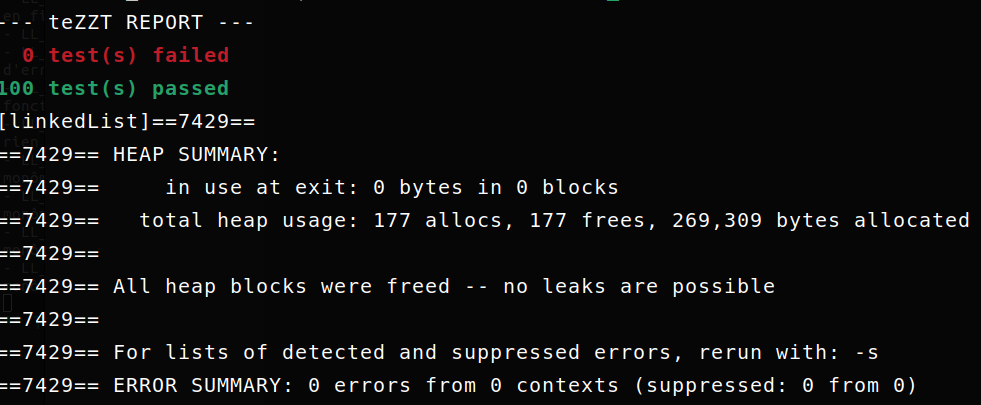
\includegraphics[width=.9\linewidth]{img/test_valgrind_linkedlist.png}
\end{center}

\subsection{Tests dans polynome\textsubscript{main}}
\label{sec:org45e626f}
Les tests présents dans \textbf{polynome\textsubscript{main.c}} permettent de tester les fonctions qui
sont codées dans \textbf{polynome.c}.

L'affichage des tests s'effectue grâce à la fonction monom\textsubscript{save2fileforpoly}, qui
respecte la sérialisation suivante : "(\%2.f, \%d)". Le fichier de test à changer
lors de la dernière séance, nous n'avons pas effectué les changements car nous
avions déjà fini l'ensemble des tests. De plus, l'affichage dépend de la fonction
donnée en paramètre, donc non-pénalisant pour les tests de l'évaluation.

Dans le fichier tests, on retrouve :
\begin{itemize}
\item LL\textsubscript{init}\textsubscript{list} : vérifie que lors de l'initialisation d'un polynôme, ce dernier
\end{itemize}
pointe vers NULL
\begin{itemize}
\item Poly\textsubscript{derive1} : vérifie la bonne dérivation avec un polynôme quelconque
\item Poly\textsubscript{derive2} : vérifie la bonne dérivation avec un polynôme possédant un
\end{itemize}
monôme de degré null
\begin{itemize}
\item Poly\textsubscript{derive3} : vérifie que la dérivation d'un polynôme NULL ne provoque pas
\end{itemize}
d'erreur
\begin{itemize}
\item Poly\textsubscript{addition0} : vérifie que l'addition est correcte entre deux polynômes avec
\end{itemize}
le même nombre de maillons et de même degrés
\begin{itemize}
\item Poly\textsubscript{addition1} : vérifie que l'addition est correcte entre deux polynômes
\end{itemize}
quand l'addition provoque la suppression d'un monôme du milieu
\begin{itemize}
\item Poly\textsubscript{addition2} : vérifie que l'addition est correcte entre deux polynômes
\end{itemize}
quand l'addition provoque la suppression du monôme en tête
\begin{itemize}
\item Poly\textsubscript{addition3} : vérifie que l'addition est correcte entre deux polynômes
\end{itemize}
quand l'addition provoque la suppression du dernier monôme 
\begin{itemize}
\item Poly\textsubscript{addition4} : vérifie que l'addition est correcte entre deux polynômes de
\end{itemize}
taille différente (dim P1 > dim P2)
\begin{itemize}
\item Poly\textsubscript{addition5} :  vérifie que l'addition est correcte entre deux polynômes de
\end{itemize}
taille différente (dim P1 > dim P2)
\begin{itemize}
\item Poly\textsubscript{addition6} : vérifie que l'addition est correcte lorsque des maillons de
\end{itemize}
P2 doivent être insérés dans P1
\begin{itemize}
\item Poly\textsubscript{addition7} : vérifie que l'addition est correcte lorsque la somme provoque
\end{itemize}
le polynôme NULL [P1 + (-1*P1)]
\begin{itemize}
\item Poly\textsubscript{addition8} : vérifie que l'addition vaut P2 lorsque P1 est NULL
\item Poly\textsubscript{addition9} : vérifie que l'addition vaut P1 lorsque P2 est NULL
\item Poly\textsubscript{addition10} : vérifie que l'addition vaut NULL lorsque P1 et P2 sont NULL
\item Poly\textsubscript{produit0} : vérifie que le produit entre deux polynômes quelconque est
\end{itemize}
correcte
\begin{itemize}
\item Poly\textsubscript{produit1} : vérifie que le produit entre P1 NULL et P2 quelconque donne un
\end{itemize}
polynôme NULL
\begin{itemize}
\item Poly\textsubscript{produit2} : vérifie que le produit entre P1 quelconque et P2 NULL donne un
\end{itemize}
polynôme NULL
\begin{itemize}
\item Poly\textsubscript{produit3} : vérifie que le produit entre P1 NULL et P2 NULL donne un
\end{itemize}
polynôme NULL, ne provoque pas d'erreur


Voici une photo prouvant qu'il n'y a pas de fuites de mémoires, ni d'erreur de
mémoire dans le fichier \textbf{polynome\textsubscript{main.c}} 
\begin{center}
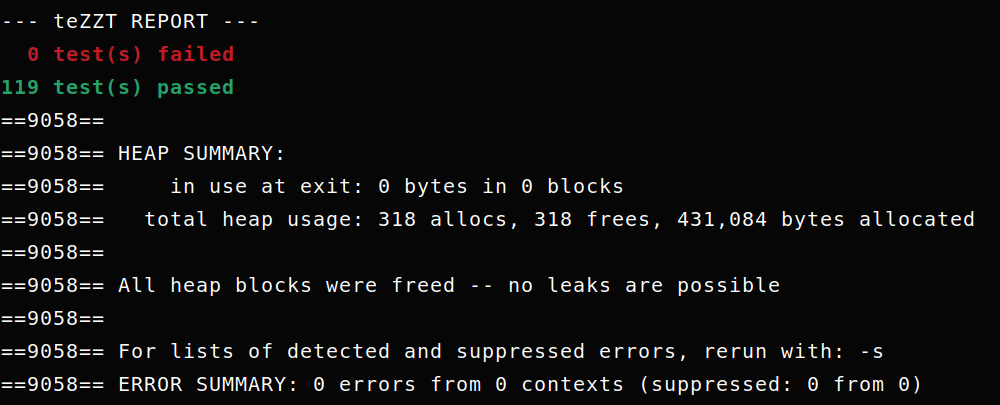
\includegraphics[width=.9\linewidth]{img/test_valgrind_polynome.png}
\end{center}
\end{document}
